```latex
\documentclass[a4paper,12pt]{article}
\usepackage[utf8]{inputenc}
\usepackage{graphicx}
\usepackage{booktabs}
\usepackage{float}
\usepackage{hyperref}
\hypersetup{
    colorlinks=true,
    linkcolor=blue,
    filecolor=magenta,      
    urlcolor=cyan,
}

\begin{document}

% Pagina iniziale senza interruzione automatica
\begin{center}
    \vspace*{1cm}
    
    \Huge
    \textbf{Progetto di Analisi: Employee Retention}
    
    \vspace{0.5cm}
    \large
    Basato sul dataset \url{https://www.kaggle.com/datasets/tawfikelmetwally/employee-dataset}
    
    \vspace{1.5cm}
    
    \textbf{Raffaele Manzo}
    
    \vfill
    
    \large
    \textbf{Matricola: 05121 16484}
\end{center}

% Rimuovi il comando \newpage qui per evitare la pagina bianca iniziale

% Indice
\tableofcontents
\newpage

\section{Introduzione}
Il progetto mira a sviluppare un modello di machine learning per risolvere un problema di classificazione binaria nel contesto della gestione delle risorse umane. In particolare, l'obiettivo è determinare se un dipendente dovrebbe rimanere nell'organizzazione o lasciarla. Questa analisi fornirà supporto strategico nella gestione dei dipendenti, aiutando a identificare i fattori chiave che influenzano il turnover e a ottimizzare la produttività aziendale.

\subsection{Obiettivo e Problema}
L'obiettivo principale del progetto è costruire un modello predittivo in grado di classificare i dipendenti in due categorie:
\begin{itemize}
    \item \textbf{0}: Il dipendente rimane nell'organizzazione.
    \item \textbf{1}: Il dipendente lascia l'organizzazione.
\end{itemize}

Il problema può essere formalizzato come una classificazione supervisionata binaria, dove la variabile target \textit{LeaveOrNot} indica la classe di appartenenza. Le caratteristiche dei dipendenti, come età, livello di istruzione, anni di esperienza, genere, e altri fattori, verranno utilizzate per addestrare il modello e fare previsioni.

\subsection{Obiettivi del Progetto}
\begin{enumerate}
    \item Analizzare e preprocessare il dataset per garantire la qualità dei dati, inclusa la gestione dei valori mancanti.
    \item Sviluppare un modello predittivo utilizzando tecniche di machine learning supervisionato.
    \item Valutare le performance del modello attraverso metriche come accuracy, precision, recall e F1-score.
\end{enumerate}

\section{Analisi dei Dati}

\subsection{Descrizione del Dataset}
Il dataset contiene informazioni sui dipendenti di un'azienda, inclusi i loro background educativi, la storia lavorativa, i dati demografici e i fattori legati all'occupazione. È stato anonimizzato per proteggere la privacy dei dipendenti, pur mantenendo informazioni utili per l'analisi della forza lavoro.

\begin{table}[H]
\centering
\begin{tabular}{ll}
\toprule
\textbf{Colonna} & \textbf{Descrizione} \\
\midrule
Education & Qualifiche educative, inclusi titolo di studio, \\ & istituzione e campo di studio \\
JoiningYear & Anno di assunzione, indica la durata del servizio \\
City & Città di base o lavoro del dipendente \\
PaymentTier & Classificazione in diverse fasce salariali \\
Age & Età del dipendente, fornisce informazioni demografiche \\
Gender & Identità di genere, utile per analisi di diversità \\
EverBenched & Indica se il dipendente è stato temporaneamente \\ & senza lavoro assegnato \\
ExperienceInCurrentDomain & Anni di esperienza nel dominio attuale \\
LeaveOrNot & Variabile target: 0 (rimane), 1 (lascia) \\
\bottomrule
\end{tabular}
\caption{Descrizione delle variabili del dataset}
\end{table}


\subsection{Formato e Caricamento del Dataset}
Il dataset è fornito in formato \texttt{CSV} (Comma-Separated Values), un formato di testo leggibile e ampiamente supportato. Questo file può essere facilmente importato in Python utilizzando librerie come \texttt{pandas}. Per questo progetto, il dataset è stato caricato e analizzato con il seguente codice:

\begin{verbatim}
import pandas as pd

# Caricamento del dataset
file_path = "Employee_with_missing.csv"
data = pd.read_csv(file_path)

# Visualizzare le prime righe del dataset
data.head()

data.info()
\end{verbatim}


\subsection{Tabella dei Tipi delle Colonne del Dataset}
\begin{table}[H]
\centering
\begin{tabular}{lll}
\toprule
\textbf{Colonna} & \textbf{Tipo}  \\
\midrule
Education & Categoriale \\
JoiningYear & Numerica  \\
City & Categoriale \\
PaymentTier & Numerica \\
Age & Numerica \\
Gender & Categoriale \\
EverBenched & Categoriale\\
ExperienceInCurrentDomain & Numerica  \\
LeaveOrNot & Numerica \\
\bottomrule
\end{tabular}
\caption{Tipi delle Colonne del Dataset}
\end{table}

\section{Analisi ed Elaborazione dei Dati}

\subsection{Variabile Dipendente}
La variabile dipendente \textit{LeaveOrNot} rappresenta il target del modello ed è una variabile binaria:
\begin{itemize}
    \item \textbf{0}: Il dipendente rimane nell'organizzazione.
    \item \textbf{1}: Il dipendente lascia l'organizzazione.
\end{itemize}

Questa variabile sarà analizzata per comprendere la distribuzione delle classi e identificare eventuali sbilanciamenti che potrebbero influire sulle performance del modello. Grafici a torta e istogrammi saranno utilizzati per visualizzare la distribuzione delle classi.

\subsection{Valori Mancanti}



Il dataset aggiornato contiene 5653 righe e 9 colonne. La presenza di valori mancanti è stata simulata per riprodurre scenari realistici e rappresenta un aspetto fondamentale della fase di preprocessing. I valori mancanti sono distribuiti casualmente in tutte le colonne del dataset:
\begin{itemize}
    \item \textbf{Education}: 108 valori mancanti.
    \item \textbf{JoiningYear}: 105 valori mancanti.
    \item \textbf{City}: 115 valori mancanti.
    \item \textbf{PaymentTier}: 104 valori mancanti.
    \item \textbf{Age}: 95 valori mancanti.
    \item \textbf{Gender}: 114 valori mancanti.
    \item \textbf{EverBenched}: 99 valori mancanti.
    \item \textbf{ExperienceInCurrentDomain}: 102 valori mancanti.
    \item \textbf{LeaveOrNot}: 118 valori mancanti.
\end{itemize}

\begin{figure}[H]
    \centering
    \includegraphics[width=0.8\textwidth]{missing_values_plot.png}
    \caption{Percentuale di Valori Mancanti nelle Colonne Selezionate}
    \label{fig:missing_values}
\end{figure}

\subsection{Gestione dei Valori Mancanti}
La gestione dei valori mancanti rappresenta una fase critica del preprocessing. Dopo un'analisi delle colonne, è stato deciso di eliminare la colonna \textit{City} in quanto ritenuta poco rilevante per il contesto del problema. La decisione si basa sul fatto che la città di lavoro non incide significativamente sui fattori chiave che determinano la permanenza o l'abbandono del dipendente. Per le altre colonne, sono state adottate le seguenti tecniche:
\begin{itemize}
    \item \textbf{Imputazione per la Media}: Per la colonna numerica \textit{Age}, i valori mancanti sono stati riempiti con la media, in quanto l'età rappresenta un attributo continuo.
    \item \textbf{Imputazione per la Moda}: Per colonne categoriali come \textit{Gender}, i valori mancanti sono stati riempiti con la moda, ossia il valore più frequente.
    \item \textbf{Creazione di una Categoria per i Valori Mancanti}: Per colonne come \textit{EverBenched}, una nuova categoria \textit{Non Definito} è stata aggiunta per rappresentare i valori mancanti.
    \item \textbf{Rimozione di Righe per le Colonne Critiche}: Le righe con valori mancanti nelle colonne \textit{JoiningYear}, \textit{PaymentTier}, \textit{LeaveOrNot} ed \textit{ExperienceInCurrentDomain} sono state eliminate per preservare l'integrità e la qualità dei dati critici.
\end{itemize}

\subsubsection{Gestione dei Valori Mancanti nelle Colonne Critiche}

Per garantire la qualità e l'affidabilità del modello di machine learning, è stata adottata la strategia di rimuovere le righe con valori mancanti nelle seguenti colonne: \textit{JoiningYear}, \textit{PaymentTier}, \textit{LeaveOrNot} ed \textit{ExperienceInCurrentDomain}. La scelta è motivata dai seguenti aspetti:

\begin{itemize}
    \item \textbf{Importanza delle Colonne per il Modello}:
    \begin{itemize}
        \item \textit{JoiningYear}: Indica la durata del servizio del dipendente, un fattore chiave per l'analisi della retention.
        \item \textit{PaymentTier}: Classifica i dipendenti in fasce salariali, una variabile fortemente correlata alla motivazione e al turnover.
        \item \textit{LeaveOrNot}: È la variabile target del modello; i valori mancanti in questa colonna renderebbero inutilizzabili quelle righe per l'addestramento.
        \item \textit{ExperienceInCurrentDomain}: Fornisce informazioni sull'esperienza nel dominio attuale, un predittore significativo delle performance e della permanenza del dipendente.
    \end{itemize}

    \item \textbf{Preservazione della Qualità del Dataset}:
    L'eliminazione delle righe con valori nulli in queste colonne garantisce che il dataset finale sia composto da dati completi e affidabili. Questo minimizza il rischio di introdurre bias nel modello.

    \item \textbf{Proporzione Ridotta di Valori Mancanti}:
    La percentuale di righe con valori mancanti in queste colonne è relativamente bassa rispetto al volume totale del dataset. Pertanto, l'impatto dell'eliminazione sarà limitato, preservando comunque un dataset sufficientemente rappresentativo.

    \item \textbf{Compatibilità con il Modello}:
    La presenza di valori nulli in queste colonne critiche potrebbe causare problemi durante il processo di addestramento del modello o richiedere strategie di gestione complesse. La rimozione rappresenta una soluzione semplice ed efficace per evitare questi ostacoli.
\end{itemize}

\subsection{Grafici Associati alla Variabile Dipendente}
Per comprendere meglio le relazioni tra la variabile dipendente e le altre variabili, saranno generati grafici esplorativi:

\begin{figure}[H]
    \centering
    \includegraphics[width=0.8\textwidth]{output(3).png}
    \caption{Distribuzione di LeaveOrNot rispetto a PaymentTier}
    \label{fig:payment_tier_vs_leave}
\end{figure}

\begin{figure}[H]
    \centering
    \includegraphics[width=0.8\textwidth]{output(2).png}
    \caption{Distribuzione dell\'anno di assunzione rispetto a LeaveOrNot}
    \label{fig:joining_year_vs_leave}
\end{figure}

\begin{figure}[H]
    \centering
    \includegraphics[width=0.8\textwidth]{output(1).png}
    \caption{Distribuzione dell\'esperienza nel dominio attuale rispetto a LeaveOrNot}
    \label{fig:experience_vs_leave}
\end{figure}


\subsection{Encoding delle Variabili Categoriali}
Le variabili categoriali saranno convertite in formato numerico per essere utilizzate nei modelli di machine learning. Verranno utilizzati i seguenti metodi:
\begin{itemize}
    \item \textbf{Label Encoding}: Per colonne binarie come \textit{EverBenched} e \textit{Gender}.
    \item \textbf{One-Hot Encoding}: Per colonne con più categorie come \textit{City} ed \textit{Education}.
\end{itemize}

Queste tecniche garantiranno che tutte le variabili siano rappresentate in un formato compatibile con gli algoritmi di machine learning.

\begin{table}[H]
\centering
\begin{tabular}{ll}
\toprule
\textbf{Feature} & \textbf{Type} \\
\midrule
JoiningYear & Numerical \\
PaymentTier & Numerical \\
Age & Numerical \\
ExperienceInCurrentDomain & Numerical \\
LeaveOrNot & Numerical \\
Education\_Bachelors & Encoded Categorical \\
Education\_Masters & Encoded Categorical \\
Education\_PhD & Encoded Categorical \\
Gender\_Female & Encoded Categorical \\
Gender\_Male & Encoded Categorical \\
EverBenched\_No & Encoded Categorical \\
EverBenched\_Yes & Encoded Categorical \\
EverBenched\_NotDefined & Encoded Categorical \\
\bottomrule
\end{tabular}
\caption{Feature del Dataset Dopo Encoding Completo e Rimozione della Colonna City}
\label{tab:feature_summary_full}
\end{table}



\subsubsection{Esempio di Codice}
Un esempio di implementazione in Python:
\begin{verbatim}
from sklearn.preprocessing import LabelEncoder, OneHotEncoder

# Label Encoding
label_encoder = LabelEncoder()
data['Gender'] = label_encoder.fit_transform(data['Gender'])
data['EverBenched'] = label_encoder.fit_transform(data['EverBenched'])

# One-Hot Encoding
data = pd.get_dummies(data, columns=['Education'], drop_first=False)
\end{verbatim}

\subsubsection{Bilanciamento della Variabile Target e Correlazione delle Feature Codificate}

Dopo aver eseguito l'encoding delle variabili categoriali, è stata effettuata l'analisi della correlazione tra tutte le variabili del dataset. La heatmap risultante è mostrata di seguito:
\begin{figure}[H]
    \centering
    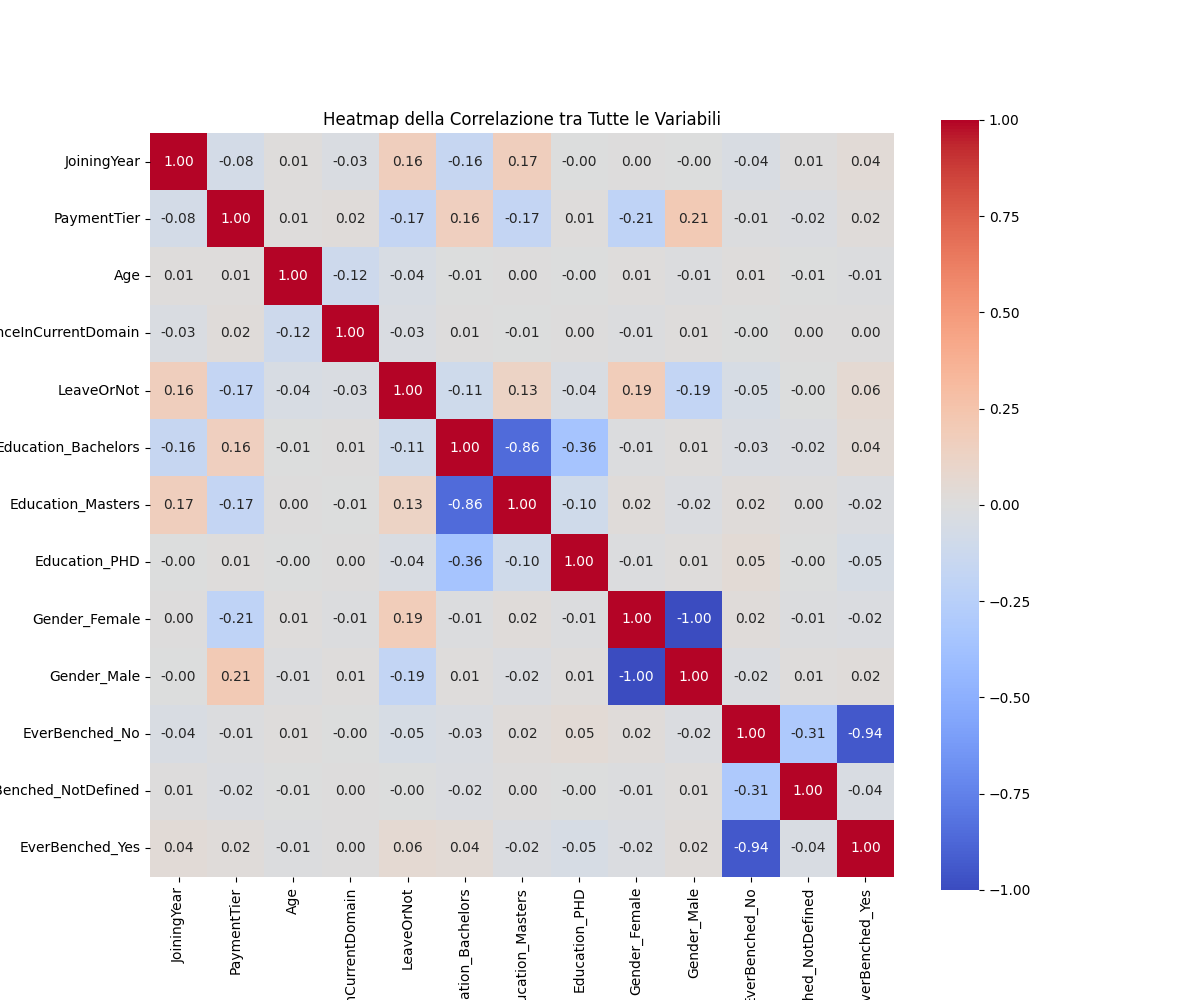
\includegraphics[width=0.9\textwidth]{heatmap_corr_vars.png}
    \caption{Heatmap della Correlazione tra Tutte le Variabili (Numeriche e Codificate)}
    \label{fig:full_correlation_heatmap}
\end{figure}

La distribuzione della variabile target \textit{LeaveOrNot} dopo l'encoding rimane invariata rispetto all'originale, come mostrato nel seguente grafico:
\begin{figure}[H]
    \centering
    \includegraphics[width=0.8\textwidth]{output(5).png}
    \caption{Distribuzione delle Classi nella Variabile Target LeaveOrNot (Dopo Encoding)}
    \label{fig:class_balance_encoded}
\end{figure}

Per bilanciare le classi durante il training, utilizzeremo la tecnica di oversampling con SMOTE, che genera nuovi dati sintetici per la classe minoritaria, mantenendo la distribuzione delle feature basata sui vicini più prossimi.

\section{Addestramento e Valutazione del Modello}

\subsection{Scelta dei Modelli}
Per affrontare il problema di classificazione binaria, sono stati selezionati due modelli da testare: la regressione logistica e Random Forest. La scelta è stata guidata da considerazioni pratiche e basate sull'obiettivo di trovare un equilibrio tra semplicità e capacità predittiva.

\subsubsection{Perché Logistic Regression?}
La regressione logistica è un modello lineare che offre una base solida per comprendere come le variabili del dataset influenzano la decisione finale. È stata scelta perché:
\begin{itemize}
    \item È intuitiva: il modello permette di interpretare facilmente il contributo di ogni variabile al risultato finale.
    \item È rapida: con dataset relativamente piccoli come il nostro, il tempo di addestramento è minimo.
    \item È affidabile: fornisce risultati chiari e prevedibili, particolarmente utili come punto di partenza per valutazioni più complesse.
\end{itemize}


\subsubsection{Perché Random Forest?}
Il modello Random Forest è stato selezionato per la sua capacità di adattarsi a problemi più complessi e gestire variabili con relazioni non lineari. Ecco perché lo consideriamo:
\begin{itemize}
    \item È versatile: riesce a catturare interazioni tra le variabili che potrebbero sfuggire a modelli più semplici.
    \item È robusto: riduce il rischio di errori gravi grazie alla combinazione di più alberi decisionali.
    \item È esplicativo: oltre a fare previsioni, fornisce una classifica dell'importanza delle variabili, utile per analisi approfondite.
\end{itemize}
Questo modello è particolarmente adatto per situazioni in cui vogliamo massimizzare l'accuratezza predittiva e ottenere una visione più dettagliata delle dinamiche del dataset.

\subsection{Valutazione dei Modelli}
Per confrontare le performance dei due modelli, utilizzeremo metriche che ci permettono di misurare sia la qualità complessiva delle previsioni sia la capacità di distinguere tra classi diverse. Le metriche selezionate sono:
\begin{itemize}
    \item \textbf{Accuracy}: Ci dice quanto spesso il modello classifica correttamente un esempio.
    \item \textbf{Precision}: Indica quanto il modello sia affidabile nel predire i casi positivi (es. predizioni di abbandono che si rivelano corrette).
    \item \textbf{Recall}: Misura la capacità del modello di individuare tutti i casi positivi, anche quelli più difficili.
    \item \textbf{F1-Score}: Una combinazione bilanciata di precision e recall, utile quando vogliamo dare uguale peso a entrambi gli aspetti.
    \item \textbf{ROC-AUC}: Fornisce una visione d'insieme sulla capacità del modello di separare correttamente le classi, indipendentemente dalla soglia utilizzata.
\end{itemize}
Queste metriche ci aiuteranno a identificare quale dei due modelli, Logistic Regression o Random Forest, sia più adatto per il nostro problema di classificazione e a prendere decisioni basate non solo sulla precisione, ma anche sull'affidabilità e sull'adattabilità del modello.

\subsection{Divisione del Dataset}

La divisione del dataset in training e test rappresenta una fase cruciale per garantire che il modello sia robusto e generalizzabile. In questa sezione, viene descritto l'approccio adottato per una divisione ottimale del dataset.


\subsubsection{Dimensione del Dataset}
Il dataset, contenente circa \textbf{5653 campioni} dopo il preprocessing, è considerato di piccole dimensioni. Pertanto, è stata adottata una divisione \textbf{80\%-20\%}, riservando l'80\% dei dati all'addestramento e il 20\% alla valutazione.

\subsubsection{Codice per la Divisione del Dataset}
Il seguente codice Python è stato utilizzato per implementare la divisione del dataset:

\begin{verbatim}
from sklearn.model_selection import train_test_split

# Divisione in training e test set (80%-20%)
X_train, X_test, y_train, y_test = train_test_split(
    X, y, test_size=0.2, random_state=42, stratify=y
)

# Verifica della distribuzione della variabile target
print("Distribuzione nel Training Set:")
print(y_train.value_counts(normalize=True))

print("\nDistribuzione nel Test Set:")
print(y_test.value_counts(normalize=True))
\end{verbatim}

\section{Valutazione dei Risultati}

\subsection{Logistic Regression}
\begin{itemize}
    \item \textbf{Senza bilanciamento}: La regressione logistica ha mostrato un'accuratezza del \textbf{65\%} e un ROC-AUC di \textbf{0.680}. Tuttavia, si evidenziano delle difficoltà nella distinzione dei dipendenti che lasciano l'azienda, con una precision per la classe minoritaria pari a \textbf{0.49} e una recall di \textbf{0.61}.
    \item \textbf{Con bilanciamento}: Dopo l'applicazione del bilanciamento con SMOTE, il modello ha registrato un lieve miglioramento nella capacità di riconoscere i dipendenti che lasciano l'azienda. Nonostante ciò, la precision è rimasta stabile (\textbf{0.50}) e la recall è leggermente diminuita (\textbf{0.55}), con un ROC-AUC di \textbf{0.668}.
\end{itemize}



\subsection{Random Forest}
\begin{itemize}
    \item \textbf{Senza bilanciamento}: Random Forest ha superato Logistic Regression con un'accuratezza del \textbf{75\%} e un ROC-AUC di \textbf{0.776}. La precision e la recall per la classe minoritaria sono rispettivamente \textbf{0.64} e \textbf{0.62}, evidenziando una capacità superiore di catturare i dipendenti che lasciano l'azienda.
    \item \textbf{Con bilanciamento}: Con l'adozione di SMOTE, Random Forest ha mantenuto una performance stabile, con un'accuratezza del \textbf{76\%} e un ROC-AUC di \textbf{0.780}. La precision per la classe minoritaria è aumentata a \textbf{0.66}, mentre la recall è rimasta stabile a \textbf{0.61}.
\end{itemize}

\begin{figure}[H]
    \centering
    \includegraphics[width=0.8\textwidth]{roc_curve.png}
    \caption{Roc Curve confrontate}
    \label{fig:confusion_rf}
\end{figure}

\subsection{Confusion Matrices}
Le matrici di confusione forniscono un quadro dettagliato dei veri positivi, falsi positivi e falsi negativi:
\begin{itemize}
    \item \textbf{Logistic Regression}: Presenta un numero elevato di falsi negativi per la classe minoritaria, indicando difficoltà nel classificare correttamente i dipendenti che lasciano l'azienda.
    \item \textbf{Random Forest}: Mostra una distribuzione più bilanciata tra veri positivi e falsi negativi, confermando una migliore capacità predittiva rispetto a Logistic Regression.
\end{itemize}


\begin{figure}[H]
    \centering
    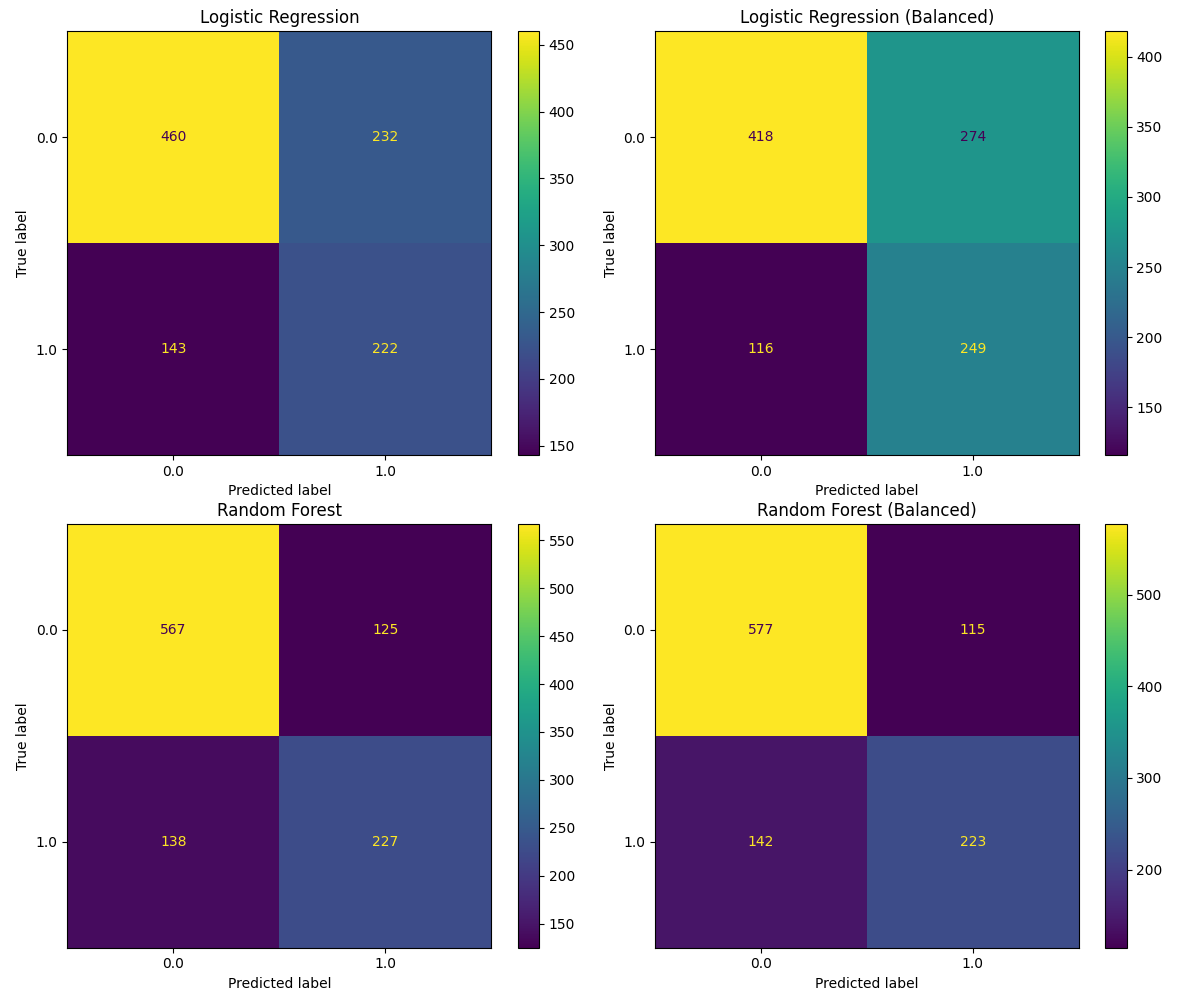
\includegraphics[width=0.8\textwidth]{conf_mat.png}
    \caption{Matrici di confusione confrontate}
    \label{fig:confusion_rf}
\end{figure}

\subsection{Tabella Riassuntiva delle Metriche}

\begin{table}[H]
\centering
\begin{tabular}{lccc}
\toprule
\textbf{Modello} & \textbf{Bilanciamento} & \textbf{Precision (1.0)} & \textbf{Recall (1.0)} \\
\midrule
Logistic Regression & No  & 0.49 & 0.61 \\
Logistic Regression & Yes & 0.50 & 0.55 \\
Random Forest       & No  & 0.64 & 0.62 \\
Random Forest       & Yes & 0.66 & 0.61 \\
\bottomrule
\end{tabular}
\caption{Metriche di Precision e Recall per Logistic Regression e Random Forest con e senza bilanciamento}
\label{tab:metrics_summary_1}
\end{table}


\begin{table}[H]
\centering
\begin{tabular}{lccc}
\toprule
\textbf{Modello} & \textbf{F1-Score (1.0)} & \textbf{Accuracy} & \textbf{ROC-AUC} \\
\midrule
Logistic Regression & 0.54 & 0.65 & 0.68 \\
Logistic Regression & 0.52 & 0.65 & 0.67 \\
Random Forest       & 0.63 & 0.75 & 0.78 \\
Random Forest       & 0.63 & 0.76 & 0.78 \\
\bottomrule
\end{tabular}
\caption{Metriche di F1-Score, Accuratezza e ROC-AUC per Logistic Regression e Random Forest con e senza bilanciamento}
\label{tab:metrics_summary_2}
\end{table}

\subsection{Considerazioni Finali}
Random Forest emerge chiaramente come il modello più adatto per questo dataset, grazie alla sua robustezza e capacità di gestire relazioni complesse tra le variabili. Sebbene la bilanciatura tramite SMOTE non abbia migliorato significativamente le metriche, si è rivelata utile per aumentare il recall della classe minoritaria.


\end{document}
```

